%!TEX encoding = UTF-8 Unicode

%!TEX root = ../compendium.tex

\ExerciseSolution{\ExeWeekNINE}


%Uppgift 1
\Task

%1.a)
\Subtask  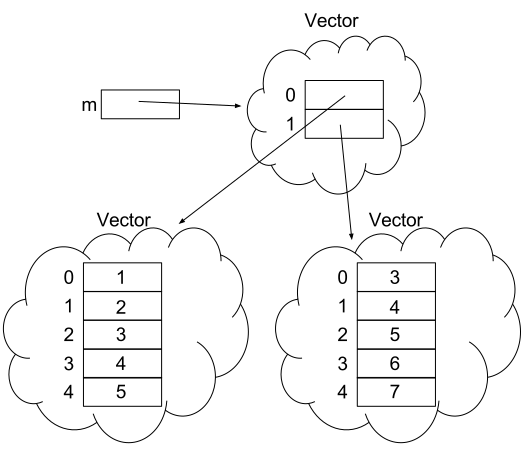
\includegraphics{../img/w09-solutions/1a} \\
Typ: \code{Vector[Vector[Int]]}\\
Värde: \code{Vector(Vector(1, 2, 3, 4, 5), Vector(3, 4, 5, 6, 7))} \\
Dimensioner: $2 \times 5$\\
Inom matematiken sker indexering enligt konvention med 1 som lägsta index. I scala är lägsta index 0, man använder s.k. 0-indexering. \footnote{Detta är inte fallet i alla programmeringsspråk, vilket du kan läsa mer om på \url{https://en.wikipedia.org/wiki/Array\_data\_type\#Index\_origin}}

%1. b)
\Subtask \\
2: \code{Int}\\
3: \code{Vector[Int]}\\
4: \code{Int}

%1.c)
\Subtask \\
m2: \code{Vector[Vector[Int]]}\\
m3: \code{Vector[Vector[AnyVal]]}\\
m4: \code{Vector[Vector[Any]]}\\
m5: \code{Vector[Vector[Int]]}

%1.d)
\Subtask TODO

%1.e)
\Subtask m5, $42 \times 2$

%Uppgift 2
\Task

%2.a)
\Subtask \begin{Code}
def throwDie: Int = (math.random * 6).toInt + 1
\end{Code}

%2.b)
\Subtask $1000 \times 5$

%2.c)
\Subtask -- %Inget svar

%2.d)
\Subtask \begin{Code}
def roll(n: Int) = Vector.fill(n)(throwDie).sorted
\end{Code}

%2.e)
\Subtask \begin{Code}
def isYatzy(xs: Vector[Int]): Boolean = xs.forall(_ == xs(0))
\end{Code}

%2.f)
\Subtask \begin{Code}
def isYatzy(xs: Vector[Int]): Boolean = {
	var foundDiff = false
	var i = 0
	while (i < xs.size && !foundDiff) {
		foundDiff = xs(i) != xs(0)
		i += 1
	}
	!foundDiff
}
\end{Code}

%2.g)
\Subtask \begin{Code}
def diceMatrix(m: Int, n: Int): Vector[Vector[Int]] =
  Vector.fill(m)(roll(n))
\end{Code}

%2.h)
\Subtask \begin{Code}
def diceMatrixToString(xss: Vector[Vector[Int]]): String =
  xss.map(_.mkString(" ")).mkString("\n")
\end{Code}

%2.i)
\Subtask Funktionen går igenom varje matrisrad, där den i sin tur går igenom
varje element på raden och lägger till i \code{StringBuilder}-objektet. Om det inte är
det sista elementet på raden läggs även ett blanktecken till, annars läggs ett
nyradstecken till. Undantaget är sista raden, där inget nyradstecken läggs till.
Slutligen konverteras \code{StringBuilder}-objektet till en \code{String} som
returneras.\\
Är \code{xss} tom utvärderas \code{0 until xss.size} till en tom \code{Range}
eftersom \code{xss.size} blir \code{0} och \code{until} är exkluderande.
Innehållet i den yttre \code{for}-loopen hoppas över och en tom sträng returneras.
Är alla rader tomma hoppas i stället de inre \code{for}-looparna över, med samma resultat.\\
Med \code{StringBuilder} behöver inte hela innehållet kopieras vid varje tillägg,
vilket spar prestanda vid många tillägg,
men eftersom det är ett föränderligt objekt kan innehållet ändras av någon annan
del av programmet som också har tillgång till referensen; objektet kan helt plötsligt
 innehålla någonting annat, trots att referensen är densamma.

%2.j)
\Subtask \begin{Code}
def filterYatzy(xss: Vector[Vector[Int]]): Vector[Vector[Int]] =
  xss.filter(isYatzy)
\end{Code}

%2.k)
\Subtask \begin{CodeSmall}
def filterYatzy(xss: Vector[Vector[Int]]): Vector[Vector[Int]] = {
	var result: Vector[Vector[Int]] = Vector()
	for (i <- 0 until xss.size) {
		if (isYatzy(xss(i))) result = result :+ xss(i)
	}
	result
}
\end{CodeSmall}

%2.l)
\Subtask --

%2.m)
\Subtask \begin{Code}
def yatzyPips(xss: Vector[Vector[Int]]): Vector[Int] =
  xss.filter(isYatzy).map(_.head)
\end{Code}


%Uppgift 3
\Task     %starts with: \emph{Strängtabell med rubrikra%%%

%3.a)
\Subtask \begin{CodeSmall}
case class Table(
	data: Vector[Vector[String]],
	headings: Vector[String],
	sep: String){

	val dim: (Int, Int) = (data.size, headings.size)

	def apply(r: Int, c: Int): String = data(r)(c)

	def row(r: Int): Vector[String]= data(r)

	def col(c: Int): Vector[String] = data.map(r => r(c))

	lazy val indexOfHeading: Map[String, Int] = headings.zipWithIndex.toMap

	def col(h: String): Vector[String] = col(indexOfHeading(h))

	def values(h: String): Vector[String] = col(h).distinct.sorted

	override lazy val toString: String =
		headings.mkString(sep) + "\n" +data.map(_.mkString(sep)).mkString("\n")
}
object Table {
	def fromFile(fileName: String, separator: Char = ';'): Table = {
		val lines = scala.io.Source.fromFile(fileName).getLines.toVector
		val matrix= lines.map(_.split(separator).toVector)
		new Table(matrix.tail, matrix.head, separator.toString)
	}
}
\end{CodeSmall}

%3.b)
\Subtask \begin{CodeSmall}
object RegTable {
 	def main( args:Array[String]): Unit = {
		val t = Table.fromFile(args(0), args(1)(1))
		val counts: Vector[Vector[String]] =
 			(0 until t.dim._2)
				.map(i => t.values(t.headings(i))
				.map(x => x + ": " + t.col(i).count(_ == x)))
				.toVector

    for (i <- 0 until t.dim._2) {
      println(s"\nColumn: ${i + 1}, ${t.headings(i)}:")
      for (j <- 0 until counts(i).length) {
        println(counts(i)(j))
      }
    }
  }
}
\end{CodeSmall}

%Uppgift 4
\Task     %starts with: \emph{Generiska funkioner.} En %%%

%4.a)
\Subtask  \begin{enumerate}
\item --
\item Strängrepresentationen av \code{42} spegelvänds
\item \code{"hej"} spegelvänds - \code{toString} av en sträng ger en likadan sträng
\item --
\item Gurk-objektets strängrepresentation spegelvänds
\item Funktionens typparameter matchar inte parameterns typ: \code{42} är ingen sträng
\item Implicit typkonvertering till \code{Double} sker för att stämma överens med typparametern, vilket ger en strängrepresentation med decimal
\end{enumerate}

%4.b)
\Subtask  \begin{enumerate}
\item En funktion definieras så att den tar emot två andra funktioner som argument, sätter ihop dem, och matar in ett tredje argument till den den sammansatta funktionen
\item En funktion som inkrementerar ett heltal med 1 definieras
\item En funktion som halverar ett flyttal definieras
\item \code{42} matas in i \code{inc()} och resultatet (\code{43}) matas vidare till \code{half()}. Inuti \code{half()} sker implicit typkonvertering till \code{Double} då talet divideras med ett flyttal (\code{2.0}) och resultatet blir \code{43.0 / 2.0}, alltså \code{21.5}.
\item Resultatet från \code{half()} är av typ \code{Double}, medan \code{inc()} tar emot ett argument av typ \code{Int}. Då flyttal generellt inte kan konverteras till heltal utan informationsförlust sker ingen implicit konvertering, istället sker ett kompileringsfel.
\end{enumerate}

%4.c)
\Subtask \begin{Code}
def inc(x: Double): Double = x + 1.0 
\end{Code}
Nu ges kompileringsfel på rad 4 istället, vilket kan lösas med följande ändring:
\begin{Code}
def half(x: Double): Double = x / 2.0 
\end{Code}


%Uppgift 4
\Task     %starts with: \emph{Generiska klasser.} Även %%%

%5.a)
\Subtask --

%5.b)
\Subtask \begin{Code}
class Cell[T](var value: T){
	override def toString = "Cell(" + value + ")"
	def concat[U](that: Cell[U]): Cell[String] =
		new Cell(value.toString + that.value.toString)
}
\end{Code}

%5.c)
\Subtask  Endast celler med samma typparameter kan nu konkateneras. Eftersom \code{concat()} returnerar ett objekt av typ \code{Cell[String]} kan ett ojämnt antal celler med någon annan typparameter än \code{String} alltså inte längre konkateneras. Är antalet jämnt går det att konkatenera dem parvis och sedan konkatenera de returnerade \code{Cell[String]}-objekten, men det är något omständigt.

%5.d)
\Subtask  --


%Uppgift 6
\Task     %starts with: \label{task:arraymatrix-java} \%%%

%6.a)
\Subtask Vid initialisering fylls alla element i \code{xss} med standardvärdet för typen, \code{0} i fallet med \code{int}. Den yttre \code{for}-loopen i \code{showMatrix()} itererar över raderna i \code{xss}. Den inre \code{for}-loopen itererar i sin tur längs med elementen på den auktuella raden och skriver ut rad, kolumn och innehåll. Efter varje rad sker en radbrytning, så att en rad i utskriften även motsvarar en rad i matrisen.\\
Exempel på skillnader mellan användning av matriser i scala och java:
\begin{itemize}
\item åtkomst: \code{minArray(rad)(kolumn)} respektive \code{minArray[rad][kolumn]}
\item typnamn: \code{Array[Array[elementTyp]]} respektive  \code{elementTyp[][]}
\item allokering: \code{Array.ofDim[typ](xDim,yDim)} respektive \code{new typ[xDim][yDim]}
\end{itemize}

%6.b)
\Subtask \begin{Code}
public class ArrayMatrix {

	public static void showMatrix(int[][] m){
		System.out.println("\n--- showMatrix ---");
		for (int row = 0; row < m.length; row++){
			for (int col = 0; col < m[row].length; col++) {
				System.out.print("[" + row + "]");
				System.out.print("[" + col + "] = ");
				System.out.print(m[row][col] + ";");
			} System.out.println();
		}
	}

	public static void fillRnd(int[][] m, int n){
		for (int row = 0; row < m.length; row++){
			for (int col = 0; col < m[row].length; col++) {
				m[row][col] = (int) (Math.random() * n + 1);
			}
		}
	}

	public static void main(String[] args) {
		System.out.println("ArrayMatrix test");
		int[][] xss = new int[10][5];
		showMatrix(xss);
		fillRnd(xss, 6);
		showMatrix(xss);
	}
}
\end{Code}


%Uppgift 7
\Task     %starts with: \emph{Skapa ett yatzy-spel för %%%

%7.a)
\Subtask  \begin{CodeSmall}
/** En skiss på en klass som kan användas till ett förenklat yatzy-spel */
case class YatzyRows(val rows: Vector[Vector[Int]]) {

	private def throwDie: Int = (math.random * 6).toInt + 1

	/** A new YatzyRows with a new row of 5 dice rolls appended to rows */
	def roll: YatzyRows = new YatzyRows(rows :+ Vector.fill(5)(throwDie))

	/** A new YatzyRow with some indices of the last row re-rolled */
	def reroll(indices: Vector[Int]): YatzyRows = 
		new YatzyRows(rows :+ rows(rows.length - 1).zipWithIndex.map {
			case (x, i) => if (indices.contains(i)) throwDie else x
		})
}
object YatzyRows {

	def isYatzy(xs: Vector[Int]): Boolean = xs.forall(_ == xs(0))

	def isThreeOfAKind(xs: Vector[Int]): Boolean = 
		xs.exists(x => xs.count(_ == x) >= 3)

	def isFourOfAKind(xs: Vector[Int]): Boolean = 
		xs.exists(x => xs.count(_ == x) >= 4)

	def isFullHouse(xs: Vector[Int]): Boolean = 
		xs.exists(x => xs.count(_ == x) == 3) &&
		xs.exists(x => xs.count(_ == x) == 2)

	def isSmallStraight(xs: Vector[Int]): Boolean = 
		xs.forall(x => xs.count(_ == x) == 1) && !xs.exists(_ == 6)

	def isLargeStraight(xs: Vector[Int]): Boolean = 
		xs.forall(x => xs.count(_ == x) == 1) && !xs.exists(_ == 1)
}

\end{CodeSmall}
Observera att fem stycken 2:or uppfyller kraven för Yatzy, men även för triss och fyrtal.

\Subtask  Slumpen gör att utfallet inte kommer stämma exakt överens med teorin, men för ett stort antal kast bör resultaten hamna ganska nära. De teoretiska sannolikheterna (utan omkast) finns i \ref{yatzyProb}.
\begin{table}[h]
\centering
\caption{Sannolikhet för olika Yatzy-resultat}
\label{yatzyProb}
\begin{tabular}{ll}
Yatzy&  $0,077\%$  \\
$\geq3$ av samma& $21\%$\\
$\geq4$ av samma& $2,0\%$\\
Kåk& $3,9\%$\\
Liten stege& $1,5\%$\\
Stor stege& $1,5\%$
\end{tabular}
\end{table}

Kodexempel:
\begin{CodeSmall}
import YatzyRows._

object YatzyStats extends App {
  val n = 1000000.0
  var yr = YatzyRows(Vector(Vector[Int]()))
  for (i <- 1 to n.toInt) yr = yr.roll
  println(s"Yatzy: ${yr.rows.count(isYatzy(_)) / n * 100}%")
  println(s"Three of a kind: ${yr.rows.count(isThreeOfAKind(_)) / n * 100}%")
  println(s"Four of a kind: ${yr.rows.count(isFourOfAKind(_)) / n * 100}%")
  println(s"Full house: ${yr.rows.count(isFullHouse(_)) / n * 100}%")
  println(s"Small straight: ${yr.rows.count(isSmallStraight(_)) / n * 100}%")
  println(s"Large straight: ${yr.rows.count(isLargeStraight(_)) / n * 100}%")
}
\end{CodeSmall}

\Subtask -- 


\Task     %%%TODO number  8 %%%starts with: \label{task:generic-matrix} \em%%%

\Subtask -- %%%TODO in task 8 %%%


\Task     %%%TODO number  9 %%%starts with: \TODO \emph{Klasser för täta oc%%%

\Subtask -- %%%TODO in task 9 %%%

\Subtask -- %%%TODO in task 9 %%%

\Subtask -- %%%TODO in task 9 %%%

\Subtask -- %%%TODO in task 9 %%%

\Subtask -- %%%TODO in task 9 %%%

\Subtask -- %%%TODO in task 9 %%%


\Task     %%%TODO number  10 %%%starts with: \emph{Matriser med \jcode{Array%%%

\Subtask -- %%%TODO in task 10 %%%
